\chapter{Expectation-maximization applied to brain segmentation}\label{sec:EM}
%Each main chapter or section should start with a short description of
%what it holds, and why. Top tip --- begin the whole writing enterprise
%with a first draft of this little bit for each chapter. It will force
%you to think about overall structure.\\get
%dsfdfs
%\par
%
Here we get going with theory of the expectation-maximization (EM) applied to brain segmentation. We show first a simple approach of the problem, in the particular case of Gaussian mixture models followed by a more generalistic approach. The simple approach will give the reader an intuitive understanding of the problem then the general approach will formalize it in order to adapt it to most of the segmentation problems. Finally, there will be a presentation of the algorithm implemented in the software suit Slicer 3 \cite{22}.
%
\section{Presentation of the EM segmentation}
%Magnetic resonance imaging (MRI) is very well suited for analyzing human soft tissue anatomy. It provides high resolution high resolution 3D volumetric data with high resolution between soft tissues. Nevertheless, this technique has some disavantages. Indeed MRI images can be alterated by some artifacts as movement, magnetic suceptibility, http://www.e-mri.org, aliasing, etc.. Another main problem is the apparition of a bias on MRIs. This bias results from QDSFQSDF. Correcting this problem is very important in the purpose of image processing. If we don't, the same tissue will have different intensities through the volume, which can bree mistakes during the segmentation process.
The EM algorithm was originally described in 1977 by Arthur Dempster, Nan Laird, and Donald Rubin\cite{1}. They generalized and developped a method used previously by authors, for specific applications. It is widely used to solve problems where data are "missing". %In our particular purpose of brain segmentation, the missing data is the knowledge of the tissues.
The EM algorithm is an iterative algorithm which works in two steps: Expectation and Maximization. It can be use to solve a lot of image processing's problems like classification, restoration\cite{3} and motion estimation\cite{2}. 
The EM segmentation has been applied to segmentation%Since the generalization of the algorithm, a lot of related papers were proposed. %Most of them bring algorithms derived from the original one to adapt it to particuliar problems, using additional informations.
\par
Nowadays, EM algorithms are become a popular tool for classification problems.  It is particulary well suited for brain MR images segmentation.
A lot of algorithms already exist. They present complex frameworks using spatial information, neighborhood or intensity inhomogeneities to enhance the classification.\\
\par
In the SPL, the algorithm developped uses spatial, tree structure arborescence and information about intensity inhomogeneity to segment the brain. 
%

\section{Background}
%
We start with a presentation of all the fundamentals the reader needs to have a good understanding of EM segmentation. We begin with a description of the statistical model used for the brain. Then we describe briefly the widely used GM model. Finally we will present what the mamixum likelihood function is. This part is mainly based on \cite{4}, \cite{5} and \cite{6}
%
\subsection{Statistical model used for the brain}
%
We define the voxel intensities of a volume as $Y=\lbrace y_1, ..., y_n\rbrace$ when the image counts $n$ voxels. $Y$ is called \textit{observed data} because this is the the data we see when we observe the image. Each $y$ is a realization of the random variable $Y$. The actual labelling of the image is $Z=\lbrace z_1, ..., z_n\rbrace$. $Z$ is called \textit{hidden data} because we do not know the value of each label. This is precisely the purpose of the segmentation: estimating the \textit{hidden data} from the observed data. We assume that the observed data is generated from the \textit{hidden data} and a parameter $\Phi$. The parameter $\Phi$ can either be a probability density function, noise,or bias field, among others, depending on the model.
\par
$Y$ and $Z$ can be viewed as $n$-dimensional random variables $Y=\lbrace Y_1, ..., Y_n\rbrace$ and $Z=\lbrace Z_1, ..., Z_n\rbrace$ then each $y_i$ is a realization of $Y_i$ and each $z_i$ is a realization of $Z_i$. The conditional probability function describing $Y_i$ is $p(Y_i|Z_i,\Phi)$.
\par
The easiest model assumes that all intensities in one class are the same, but these intensities are corrupted by factors like noise modelled by a Gaussian distribution. We can describe the relationship as below:
  
  \begin{equation*}
  y_i=\mu_k+n_i\\
  \end{equation*}

\par
where $\mu_k$ is the mean intensity of the $k^{th}$ tissue and $n_i$ a random sample generated by the corrupting factor(s). Let's say that $n_i$ is generated by a Gaussian probability distribution function $G(.,0,\sigma)$, with $0$ mean and $\sigma$ variance. That means that $y_i$ is a random sample generated by a Gaussian probability density function $G(.,\mu_k,\sigma)$. Let's assume that each class has a different variance, $G(.,\mu_k,\sigma)$ becomes $G(.,\mu_k,\sigma_k)$ and it leads to:
  
  \begin{equation}\label{CDP}
  p(y_i|Z_i=k,\Phi)=G(y_i,\mu_k,\sigma_k)\\
  \end{equation}

\par
As the labelling is not known, it is usefull to express the probability density function (PDF) of $Y_i$ only depending on parameter $\Phi$ with the total probability theorem:

  \begin{equation}\label{PDF}
  p(y_i|\Phi)=\sum_{k=1}^K p(y_i|Z_i=k,\Phi)p(Z_i=k|\Phi)\\
  \end{equation}

\par
$p(Z_i=k|\Phi)$ is the \textit{prior probability}. It expresses the probability that a voxel $i$ belongs to a class $k$. $p(y_i|Z_i=k,\Phi)$ is the \textit{likelihood}. In our case, we will assume that the \textit{prior probability} is unique for each each label. The new model we obtain for the labelling is a widely used one: the \textit{gaussian mixture model}.
%
\subsection{Gaussian mixture model}
Let's remind the first hypotesis: the conditional probability function for each tissue to segment is defined as in Equation \ref{CDP}. Moreover, we will assume that \textit{prior probability} is a constant $c_k$ for each class $k$. $c_k$ is the weight of the class $k$.
  
  \begin{equation}\label{CW}
  p(Z_i=k|\Phi)=c_k\\
  \end{equation}

The last assumption will be that $\Phi$ contains unknown means, variances and weights for each tissue. Then we can express $\Phi$ as a set of parameters such as $\Phi=(\mu_1, \sigma_1, c_1, ..., \mu_K, \sigma_K, c_K)$. %$\Phi_k$ is a sample of $\Phi$ and $\Phi_k = (\mu_k, \sigma_k, c_k)$
\par
Using Equations \ref{CDP} and \ref{CW}, Equation \ref{PDF} becomes:
 
  \begin{equation}\label{GMM}
  p(y_i|\Phi)=\sum_{k=1}^K G(y_i,\mu_k,\sigma_k)c_k\\
  \end{equation}

\par
In the case of GM model, each voxel is considered to be independent. That means that each voxel will have its own probability density function. Consequently, the normalized histogram of the whole volume can be interpreted as an approximation of the sum of all the probability density functions. %The next step is then to find the set $(\mu_i, \sigma_i, c_i)$ of parameter $\Phi$  for each voxel, to fit as well as possible the normalized histogram. A convenient way to find it is to use the \textit{Maximum likelihood} principle.
%
\subsection{Maximum likelihood}
In our case, we know the intensity of each observed voxel $y_i$. $\Phi$ are to be found. The best estimation of $\Phi$ will be obtain using the maximum likelihood principle. $p(y_i|\Phi)$ is called likelihood function. For each value of $\Phi$ it returns the value of the likelihood of $y_i$, given $\Phi$.
\par
The voxels are considered to be independent. Through the whole volume, it leads to:
 
  \begin{equation}\label{ML}
  p(Y|\Phi)= \prod_{i=1}^n p(y_i|\Phi)\\
  \end{equation}

\par
The objective is to find the parameter $\Phi$ which will maximize the likelihood of the observed volume. We can note this parameter:
  
  \begin{equation}\label{AR}
  \hat{\Phi}=\operatorname*{arg\,max}_\Phi p(Y|\Phi)\\
  \end{equation}

\par
Therefore, it is more convenient to work with logarithm because the product from Equation \ref{ML} will be converted into a summation. Equation \ref{AR} becomes:
  
  \begin{equation*}\label{ARL}
  \hat{\Phi}=\operatorname*{arg\,max}_\Phi \operatorname*{log} p(Y|\Phi). %=\operatorname*{arg\,max}_\Phi L(\Phi)\\
  \end{equation*}
  
With Equation \ref{PDF}, let us denote:

  \begin{align*}
  L(\Phi) &\triangleq \operatorname*{log} p(Y|\Phi) \\
          &= \sum_{i=1}^n \operatorname*{log} \sum_{k=1}^K p(y_i|Z_i=k,\Phi)p(Z_i=k|\Phi)\\
  \end{align*} 

Finally, in case of GM model, with Equation \ref{GMM}, $L(\Phi)$ becomes:
  
  \begin{equation*}\label{LP}
  L(\Phi)=\sum_{i=1}^n \operatorname*{log} \sum_{k=1}^K G(y,\mu_k,\sigma_k)c_k\\
  \end{equation*}

The $log$ likelihood can be maximized by finding partial derivatives for each parameter. When the partial derivative of $L(\Phi)$ is $0$ for a parameter, we have the maximum likelihood for the parameter $\Phi$.
\par
For example, to find the maximum likelihood regarding $\mu_k$ we first have to find when:

  \begin{equation*}\label{PD}
  \frac{\partial}{\partial\mu_k}(L(\Phi))=0\\
  \end{equation*}

\par
Then we compute the partial derivative of $L(\Phi)$ over $\mu_k$:
%\begin{equation}\label{PDF}

  \begin{align}\label{partialDerivative}
  \frac{\partial}{\partial\mu_k}(L(\Phi)) &= \frac{\partial}{\partial\mu_k}( \sum_{i=1}^n \operatorname*{log} \sum_{k=1}^K G(y_i,\mu_k,\sigma_k)c_k\nonumber)  \\
                                          &= \sum_{i=1}^n \frac{G(y_i,\mu_k,\sigma_k)c_k}{\sum_{j=1}^K G(y_i,\mu_j,\sigma_j)c_j}\frac{\partial}{\partial\mu_k}  (-\frac{(y_i-\mu_k)^2}{2\sigma_k^2}) \nonumber \\
                                          &= \sum_{i=1}^n \frac{G(y_i,\mu_k,\sigma_k)c_k}{\sum_{j=1}^K G(y_i,\mu_j,\sigma_j)c_j}(\frac{(y_i-\mu_k)}{\sigma_k^2}) \nonumber \\
                                          &= \sum_{i=1}^n \frac{p(y_i|Z_i=k,\Phi)p(Z_i=k|\Phi)}{\sum_{j=1}^K p(y_i|Z_i=j,\Phi)p(Z_i=j|\Phi)}(\frac{(y_i-\mu_k)} {\sigma_k^2})
  \end{align}

%\end{equation}
%Let's introduce the \textit{posterior probability}. It expresses the probability that a voxel belongs to a tissue. It is also called \textit{soft assignement} of %\textit{soft segmentation}. The probability that a pixel $i$ belongs to a class $j$ is:
% \begin{equation}\label{PP}
%  p(Z_i=j|Y_i=y_i,\Phi)
%  \end{equation}
Using Bayes' theorem (see App.~\ref{app:formulas}, Sec.~\ref{f:Bayes}), we notice that:

  \begin{equation}\label{BF}
  p(Z_i=k|y_i,\Phi)= \frac{p(y_i|Z_i=k,\Phi)p(Z_i=k|\Phi)}{\sum_{j=1} p(y_i|Z_i=j,\Phi)p(Z_i=j|\Phi)}\\
  \end{equation}

Thus, setting the denominator to 0 in Equation \ref{partialDerivative} and using Equation \ref{BF} yields:
 
  \begin{equation}\label{YY}
  \sum_{i=1}^n p(Z_i=k|y_i,\Phi)(y-\mu_k)=0\\
  \end{equation}

%The \textit{posterior probability} helps us to define the \textit{probability map}.
Let us denote

  \begin{equation}%\label{}
  p_{ik}=p(Z_i=k|y_i,\Phi)\\
  \end{equation}

Equation \ref{YY} leads to:
 
  \begin{equation}\label{MU}
  \mu_k = \frac{\sum_{i=1}^n y_ip_{ik}}{\sum_{i=1}^n p_{ik}}\\
  \end{equation}
Proceeding the same way as we did for Equation \ref{YY}, we can get similar equations for variance $\sigma_k$ and weight $c_k$. 

We find that:

  \begin{equation}\label{SI}
  \sigma_k^2 = \frac{\sum_{i=1}^n (y_i-\mu_k)^2p_{ik}}{\sum_{i=1}^n p_{ik}}\\
  \end{equation}
  
  \begin{equation}\label{WE}
  c_k = \frac{1}{n}\sum_{i=1}^n p_{ik}\\
  \end{equation}

\par
Equations \ref{MU},\ref{SI} and \ref{WE} provides us
  \begin{equation}\label{SS}
  p_{ik}= \frac{G(y_i,\mu_k,\sigma_k)c_k}{\sum_{j=1}^K G(y_i,\mu_j,\sigma_j)c_j}\\
  \end{equation}


This equation expresses that a voxel $i$ belongs to the class $k$. It is formulation for soft segmentation. $p_{ik}$ is called soft assignment.
$p_{ik}$ is used to fill a "map" of soft segmentation. At the end of the segmentation process, this map contains the probability that the voxel $i$ belongs to class $1, 2, ..., K$. We determine the class of the voxel $i$ looking at the class which has the highest probability in the map for this given voxel $i$.
  
\par
The segmentation can now be calculated following an iterative process called \textit{expectation maximization}.
%
\section{Expectation maximization algorithm}
The EM algorithm is a method to find the maximum likelihood for a given set of parameter ($\Phi$ in our case). Here we start with an 
intuitive description of the algorithm in the particular case of Gaussian mixture model then we will present a more general definition.
%
\subsubsection{Algorithm in case of Gaussian mixture data model}
Let's assume that we can find the maximum likelihood of the hidden data by a direct differentiation (because of the Gaussian mixture model). The EM algorithm is an iterative process of two steps: the expectation step (E-Step) and the maximization step (M-Step). At each iteration, the maximum likelihood will be increased until convergence is reached.\\
\begin{itemize}

\item \textbf{E-step}\\
In this step, we calculate an estimation of soft segmentation $p^{(m+1)}$ with Equation \ref{SS} as below. We know all the variables needed for the calculation from the observed data and the current parameter estimate $\Phi^{(m)}$. Note that an initialization is necessary for the first iteration.\\

  \begin{equation*}
  p_{ik}^{(m+1)}= \frac{G(y_i,\mu_k^{(m)},\sigma_k^{(m)})c_k^{(m)}}{\sum_{j=1}^K G(y_i,\mu_j^{(m)},\sigma_j^{(m)})c_j^{(m)}}\\
  \end{equation*}

\item \textbf{M-step}\\
In this step, we estimate the maximum likelihood for parameter $\Phi^{(m+1)}$. We do it with Equations \ref{MU},\ref{SI} and \ref{WE} as below. We know all the variables needed for the calculation from the observed data and the current estimate $p^{(m+1)}$ of hidden data.\\

  \begin{equation*}
  \mu_k^{(m+1)} = \frac{\sum_{i=1}^n y_ip_{ik}^{(m+1)}}{\sum_{i=1}^n p_{ik}^{(m+1)}}\\
  \end{equation*}

  \begin{equation*}
  (\sigma_k^{(m+1)})^2 = \frac{\sum_{i=1}^n (y_i-\mu_k^{(m+1)})^2p_{ik}^{(m+1)}}{\sum_{i=1}^n p_{ik}^{(m+1)}}\\
  \end{equation*}
  
  \begin{equation*}
  c_k^{(m+1)} = \frac{1}{n}\sum_{i=1}^n p_{ik}^{(m+1)}\\
  \end{equation*}
\end{itemize}

%EM algorithm iterates until convergence is reached. 
%As discussed in \cite{7} , convergence is assured since the algorithm is guaranted to increase the likelihood at each iteration.
The problem is simple as long as we are working with Gaussian mixture model. In the other case, the log-likelihood can not be maximized by direct differentiation and a generalized approach must be used.
%
\subsubsection{Generalized algorithm}\label{GENERAL}
Now we assume that we are no longer working with Gaussian mixture model. Thus, we must use a more general algorithm. %We will first present briefly the E-Step and the M-Step. Then we will explain the function used in both steps and finally we will show how we can use it for the specific problem of segmentation.\\
To explain the general algorithm, we will start from the log-likelihood $L(\Phi)$. As presented in the previous subsection, we wish to find $\Phi$ such as $p(Y|\Phi)$ is a maximum. We have:

  \begin{equation*}
  L(\Phi)=\operatorname*{log} p(Y|\Phi)\\
  \end{equation*}
 
Since $log$ is a strictly increasing function, the value of $\Phi$ which maximizes  $p(Y|\Phi)$ also maximizes $L(\Phi)$. Assume that after the $m^{th}$ iteration, the current estimate of $\Phi$ is given by $\Phi^{(m)}$. Since the objective is to maximize $L(\Phi)$ we want an updated estimate $\Phi$ such that

  \begin{equation*}
  L(\Phi)>L(\Phi^{(m)})
  \end{equation*}
 
In other words, we want to maximize the difference $L(\Phi)-L(\Phi^{(m)})$. For convenience, we introduce a new variable $z_{ik}$ which means that $Z_i=k$. Using the new notation, we can transform this difference as below:

 
  \begin{align*}
  L(\Phi)-L(\Phi^{(m)}) &=\operatorname*{log} p(Y|\Phi) -\operatorname*{log} p(Y|\Phi^{(m)})\\
                    &=\sum_{i=1}^n\{\operatorname*{log} \sum_{k=1}^K p(y_i|z_{ik},\Phi)p(z_{ik}|\Phi)-\operatorname*{log} p(y_i|\Phi^{(m)})\}\\
                    &=\sum_{i=1}^n\{\operatorname*{log} \sum_{k=1}^K p(y_i|z_{ik},\Phi)p(z_{ik}|\Phi).\frac{p(z_{ik}|y_i,\Phi{(m)})}{p(z_{ik}|y_i,\Phi^{(m)})}-\operatorname*{log} p(y_i|\Phi{(m)})\}\\
                    &=\sum_{i=1}^n\{\operatorname*{log} \sum_{k=1}^K p(z_{ik}|y_i,\Phi^{(m)}).\frac{p(y_i|z_{ik},\Phi)p(z_{ik}|\Phi)}{p(z_{ik}|y_i,\Phi_n)}-\operatorname*{log} p(y_i|\Phi_n)\}\\
                    &\geq \sum_{i=1}^n\{\sum_{k=1}^K p(z_{ik}|y_i,\Phi^{(m)})\operatorname*{log} \frac{p(y_i|z_{ik},\Phi)p(z_{ik}|\Phi)}{p(z_{ik}|y_i,\Phi^{(m)})}-\operatorname*{log} p(y_i|\Phi^{(m)})\}
  \end{align*}

We can deduce this inequality from Jensen's inequality (see App.~\ref{app:formulas}, Sec.~\ref{f:Jensen}) since  $p(z_{ik}|y_i,\Phi^{(m)})$ is a probability mesure and $log$ a concave function (\cite{5}). %Indeed, 

%  \begin{equation*}
%  p(z_{ik}|Y_i,\Phi_n)>0\\
%  \end{equation*}
%  \begin{equation*}
%  \sum_k p(z_{ik}|Y_i,\Phi_n)=1\\
%  \end{equation*}
\par
We will then use the fact that  $\sum_k p(z_{ik}|y_i,\Phi^{(m)})=1$. In this case, it leads to $\operatorname*{log} p(Y|\Phi^{(m)})=\sum_k p(z_{ik}|y_i,\Phi^{(m)})\operatorname*{log} p(Y|\Phi^{(m)})$. This allows us to bring $\operatorname*{log} p(Y|\Phi^{(m)})$ into the summation. 
\par
We will also use a new variable $e_k$ to express the difference through the whole volume without a summation. $e_k$ is defined as $e_k=\{z_{1k}, ..., z_{nk}\}$ when the image consists of $n$ voxels. For example, $z_{ik}=e_k=\{0,...,0,1,0,...,0\}$ means that voxel $i$ belongs to class $k$.

  \begin{align*}
  L(\Phi)-L(\Phi^{(m)}) &\geq \sum_{i=1}^n\{\sum_{k=1}^K p(z_{ik}|y_i,\Phi^{(m)})\operatorname*{log} \frac{p(y_i|z_{ik},\Phi)p(z_{ik}\Phi)}{p(z_{ik}|y_i,\Phi^{(m)})}-\operatorname*{log} p(Y|\Phi^{(m)})\} \\
                    &=\sum_{i=1}^n\{\sum_{k=1}^K   p(z_{ik}|y_i,\Phi^{(m)})\operatorname*{log} \frac{p(y_i|z_{ik},\Phi)p(z_{ik}|\Phi)}{p(z_{ik}|y_i,\Phi^{(m)})p(y_i|\Phi^{(m)})}\}\\
                    &=\sum_{k=1}^K   p(e_{k}|Y,\Phi^{(m)})\operatorname*{log} \frac{p(Y|e_{k},\Phi)p(e_{k}|\Phi)}{p(e_{k}|Y,\Phi^{(m)})p(Y|\Phi^{(m)})}\\
                    &\triangleq \Delta(\Phi|\Phi^{(m)})
  \end{align*}

We can then conclude that:

  \begin{align*}
  L(\Phi) &\geq L(\Phi^{(m)}) + \Delta(\Phi|\Phi^{(m)})\\
          &\geq l(\Phi|\Phi^{(m)})
  \end{align*}

where $l(\Phi|\Phi^{(m)}) \triangleq  L(\Phi{(m)}) + \Delta(\Phi|\Phi^{(m)})$.\\
\par
We have now a function $l(\Phi|\Phi^{(m)})$ which is bounded above by $L(\Phi)$. Additionnaly, we observe that $(l(\Phi^{(m)},\Phi^{(m)}))=L(\Phi^{(m)})$. \\
%From equation ~(\ref{ineq}), we deduce that each $\Phi$ which increases $l(\Phi|\Phi_n)$ will increase $L(\Phi)$ too.
\par
Our objective is to choose values of $\Phi$ which will maximize $L(\Phi)$. We have shown that the function $l(\Phi,\Phi^{(m)})$ is bounded above by the likelihooh function $L(\Phi)$. Moreover, the value of $\Phi$ for which the function $(l(\Phi,\Phi^{(m)}))$ and $L(\Phi)$ are egals is $\Phi=\Phi^{(m)}$. Therefore, any $\Phi$ which will increase $l(\Phi,\Phi^{(m)})$ will increase $L(\Phi)$. In order to maximize $L(\Phi)$ as much as possible, we maximize $L(\Phi)$ such as: $L(\Phi{(m)})=l(\Phi^{(m)},\Phi^{(m)})<l(\Phi^{(m+1)},\Phi^{(m)})<L(\Phi^{(m+1)})...$. As soon as $L(\Phi{(m+1)})<L(\Phi{(m)})$, the convergence has been reached and the maximum likelihood found. 
We can formalize this search. $\Phi^{(m+1)}$ is the updated value which is found after maximization of $\Phi$ using $\Phi^{(m)}$. %Once $\Phi^{(m)}=\Phi^{(m+1)}$, the algorithm has converged.

  \begin{align}\label{eMF}
  \Phi^{(m+1)} &= \operatorname*{arg\,max}_\Phi \{l(\Phi|\Phi^{(m)})\} \nonumber \\         
             &= \operatorname*{arg\,max}_\Phi \{L(\Phi^{(m)}) + \sum_{k=1}^K   p(e_{k}|Y,\Phi^{(m)})\operatorname*{log} \frac{p(Y|e_{k},\Phi)p(e_{k}|\Phi)}{p(e_{k}|Y,\Phi^{(m)})p(Y|\Phi^{(m)})}\} \nonumber \\
             &\mbox{As $p(e_{k}|Y,\Phi^{(m)})$ and $p(Y|\Phi^{(m)})$ do not depend on $\Phi$} \nonumber \\
             %&{now we remove the terms which are constants regarding \Phi }\\
             &=\operatorname*{arg\,max}_\Phi \{\sum_{k=1}^K   p(e_{k}|y_i,\Phi^{(m)})\operatorname*{log} p(Y|e_{k},\Phi)p(e_{k}|\Phi) \} \nonumber \\
             &=\operatorname*{arg\,max}_\Phi \{\sum_{k=1}^K   p(e_{k}|Y,\Phi^{(m)})\operatorname*{log} \frac{p(Y,e_{k},\Phi)p(e_{k},\Phi)}{p(e_{k},\Phi)p(\Phi)}\}      \nonumber \\
             &=\operatorname*{arg\,max}_\Phi \{\sum_{k=1}^K   p(e_{k}|Y,\Phi^{(m)})\operatorname*{log} p(Y,e_{k}|\Phi)\} \\
             &=\operatorname*{arg\,max}_\Phi \{ E_{Z|Y,\Phi^{(m)}} \{\operatorname*{log} p(Y,Z|\Phi)\}\} \nonumber
  \end{align}
  
We notice from Equation \ref{eMF}, that for a given voxel $i$:

  \begin{equation}\label{BAYES}
  \sum_{k=1}^K   p(e_{k}|y_i,\Phi^{(m)})\operatorname*{log} p(y_i,e_{k}|\Phi) = \sum_{k=1}^K   p_{ik}^{(m+1)}\operatorname*{log} p(y_i,e_{k}|\Phi)
  \end{equation}

Now, both expectation and maximization steps are apparents.\\
\begin{itemize}
\item \textbf{E-step}\\
This is the expectation step. During this step, we estimate the probability that the pixel $i$ belongs to class $k$ regarding $\Phi_{(m)}$. This equation is obtained from Equation \ref{BAYES} with Bayes formula.

  \begin{equation}\label{ESTEP1}
  p_{ik}^{(m+1)} = \frac{p(y_i|e_k,\Phi^{(m)})p(e_k|\Phi^{(m)})}{\sum_{j=1}^K   p(y_i|e_j,\Phi^{(m)}) p(e_{j}|\Phi^{(m)})}  
  \end{equation}

Using this probability, $E_{Z|Y,\Phi^{(m)}}$ returns the expected value of the parameter $\Phi$ regarding $\Phi^{(m)}$.\\


\item \textbf{M-step}\\
This is the maximization step. During this step $\operatorname*{arg\,max}_\Phi$ maximizes $E_{Z|Y,\Phi^{(m)}}$ for the parameter $\Phi$. It returns $\Phi^{(m+1)}$
  \begin{equation}
  \operatorname*{arg\,max}_\Phi \{ E_{Z|Y,\Phi^{(m)}} \{\operatorname*{log} p(Y,Z|\Phi)\}\}\\
  \end{equation}
 
\end{itemize} 
  
The EM algorithm iterates until convergence is reached. The condition of convergence can differ from an algorithm to another. A possibility is to fix the number of iterations, $C$, of the algorithm. Most of the time, the following approach is used; convergence is reached when the difference between the estimation of the parameter $\Phi$, at step $m$ and step $m+1$ is smaller than $\varepsilon$:

  \begin{equation*}
  \Phi^{(m+1)}-\Phi^{(m)} < \varepsilon
  \end{equation*}

If after the $C^{th}$ iteration, this condition is not satisfied, the EM algorithm is stopped. \\

 
  \par
  We are now familiar with the theory behind the EM algorithm. The logic appears and we can summarize the basic algorithm with the Figure \ref{fig:EMAlgorithm}:
   
  \begin{figure}[ht]\centering
  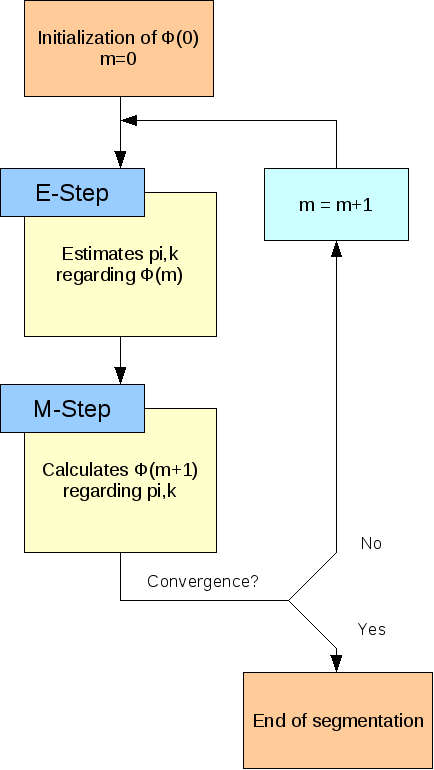
\includegraphics[width=.4\textwidth]{Images/Graphics/EMSimple.png}
  \caption{Illustration of the basic EM algorithm}\label{fig:EMAlgorithm}
  \end{figure}

\section{Expectation maximization algorithm used in Slicer 3}\label{angels}
In this part, we present the EM algorithm which has been developped in Slicer 3 and the pipeline in which it has been integrated as well. Finally, we briefly discuss the limitations of this one.
\par
The EM algorithm which is used in the SPL is derived from the original one. It enhances the original algorithm by the addition of informations like a probalistic atlas, a multichannel segmentation, a bias correction and a structure information. In Slicer 3, the Gaussian mixture model is used to describe the tissues to segment. Thus it will simplify the problem and the notations.
%
\subsection{Probabilistic atlas}\label{spatial}
The EM algorithm is very sensitive to initialization since it only finds local extremums during the maximization step. A solution to enhance the initialization is to use atlases. An atlas is needed for each tissue the user wants to segment. For each voxel $i$ of the volume, the atlas returns the probability that this voxel belongs to class $k$. This probability can be used as initialization.
  \begin{equation*}
  p_{ik}^{(0)} = p_{ik}^{atlas}
  \end{equation*}   

From this value, it estimates $\Phi^{(1)}$ and the algorithm iterates until convergence is reached. The probabilistic atlases are not only used to inialize the process. It is also use to get a more robust algorithm. Indeed, we can use the spatial information given by the atlases. Voxels will be classified not only based on intensity but regarding spatial position too. Van Lemput \textit{et al.} (\cite{8} and \cite{9}) used the spatial prior at each iteration. It is constant and we then have a spatial information. The probability that a pixel $i$ belongs to class $k$, in the E-Step changes. From Equation \ref{ESTEP1}, it becomes:

  \begin{equation*}\label{ESTEP2}
  p_{ik}^{(m+1)} = \frac{p(y_i|e_k,\Phi^{(m)}p_{ik}^{atlas}}{\sum_{j=1}^K   p(Y_i|e_j,\Phi^{(m)}) p_{ik}^{atlas}}  
  \end{equation*}

%
\subsection{Multichannel segmentation}\label{multichannel}
Most of the time, several sequences of a given modality are used to process brain segmentation. Indeed, the best suited sequence to use depends on the tissue you want to segment. For example, MR images provided by T1 sequences \cite{12} are well suited to segment white matter (WM) but are not accurate for cerebrospinal fluid (CSF). On the contrary, T2 sequences \cite{12} MR images which are well suited for CSF and not for WM. To formalize the utilization of different MR images sequence (i.e. different channels)s during the segmentation, we will change the definition of $y_i$, $\mu_k$ and $\sigma_k$ we did at the beginning. Let $y_i = \{y_{i1},y_{i2}, ..., y_{iR}\}$, $\mu_k = \{\mu_{k1},\mu_{k2}, ..., \mu_{kR}\}$ and $\sigma_k = \{\sigma_{k1},\sigma_{k2}, ..., \sigma_{kR}\}$ when we use $R$ channels, from different modalities to do the segmentation. The equations for the E-Step and the M-Step will remain the same.
%
\subsection{Bias field correction}\label{biasfield}
A major issue in MR modality is that the images can be corrupted by a low field bias field. It is mainly due to equipment limitations and to patient induced electrodynamic interactions (\cite{12}). We will now present how this bias field can be estimated and corrected in the EM algorithm.
%
\subsubsection{Principle}
Let $I=(I_1, ..., I_n)$ the observed intensities in an image, $I^*=(I_1^*, ..., I_n^*)$ the ideal intensities and $F=(F_1, ..., F_n)$ the bias field. We use the assumption that the bias field is only multiplicative. Degradation of each voxel can then be expressed as:

  \begin{equation*}
  I_i=I_i^*F_i
  \end{equation*}

Let $Y=(Y_1, ..., Y_n)$ and $Y^*=(Y_1^*, ..., Y_n^*)$ be the log-transformed observed and ideal intensities.$B=(B_1, ..., B_n)$ the log-bias field. This transform makes the bias field become additive instead of multiplicative without the log-approach.

  \begin{equation*}
  Y_i=Y_i^* + B_i
  \end{equation*}
  
We can model the PDF of the voxel intensity with a Gaussian distribution

 \begin{equation*}
  p(y_i|e_k, \Phi, B) = G(y_i-b_i,\mu_k,\sigma_k)
  \end{equation*}
  
The low frequency characteristic of the bias field $B$ can be modeled by a linear combination of smooth basic functions $\Psi_l(x)$ (\cite{13}). Let $b_i$ be the realization of the random variable $B_i$ 

  \begin{equation*}
  b_i = \sum_{l=1}^L a_l\Psi_l(pos(i))
  \end{equation*}
  
 $pos(i)$ returns the 3D position $(x,y,z)$ of the voxel $i$. $a_i$ is the $i^{(th)}$ value of the vector $A=(a_1, ..., a_L)$. $A$ represents the bias field parameters.
 \par
In the Gaussian model, bias field can then be estimated using EM framework. The bias field parameter $A$ will be used during the E-Step , through $b_i$ to estimate the soft segmentation. $A$ will be re-estimated during the M-Step, after the maximization of the tissue class parameters (mean, variance and weight).
Van Leemput formalised the two steps as below (\cite{8} and \cite{9}):\\

%\par
\begin{itemize}

\item\textbf{E-step}\\
  \begin{equation*}
  p_{ik}^{(m+1)}= \frac{G(y_i-b_i,\mu_k^{(m)},\sigma_k^{(m)})p_{ik}^{atlas}}{\sum_{j=1}^K G(y_i-b_i,\mu_j^{(m)},\sigma_j^{(m)})p_{ij}^{atlas}}\\
  \end{equation*}
  
%\par
\item\textbf{M-step}\\
  \begin{itemize}

  \item Gaussian distribution parameters estimation
    
    \begin{equation*}
    \mu_k^{(m+1)} = \frac{\sum_{i=1}^n y_ip_{ik}^{(m+1)}-b_i}{\sum_{i=1}^n p_{ik}^{(m+1)}}\\
    \end{equation*}

    \begin{equation*}
    (\sigma_k^{(m+1)})^2 = \frac{\sum_{i=1}^n (y_i-\mu_k^{(m+1)}-b_i)^2p_{ik}^{(m+1)}}{\sum_{i=1}^n p_{ik}^{(m+1)}}\\
    \end{equation*}

  \item Bias field correction

  \begin{equation}\label{BIASFIELD}  
  (A^{(m+1)})^T = (F^TW^{(m+1)}F)^{-1}F^TW^{(m+1)}R^{(m+1)}  
  \end{equation}

with:

  \begin{equation*}
   \mathbf{F} = \left(
  \begin{array}{clcr}
   \Psi_1(pos(1)) & \Psi_2(pos(1)) & \ldots & \Psi_L(pos(1)) \\
   \Psi_1(pos(2)) & \Psi_2(pos(2)) & \ldots & \Psi_L(pos(2)) \\
   \vdots & \vdots & \ddots \\
   \Psi_1(pos(N)) & \Psi_2(pos(N)) & \ldots & \Psi_L(pos(N)) \\
  \end{array} \right)
  \end{equation*}
  
  \begin{equation*}
   \mathbf{W^{(m+1)}} = \left(
  \begin{array}{clcr}
   \sum_{k=1}^K w_{1k}^{(m+1)} & 0 & \ldots & 0 \\
   0 & \sum_{k=1}^K w_{2k}^{(m+1)} & \ldots & 0 \\
   \vdots & \vdots & \ddots \\
   0 &  \ldots & 0 & \sum_{k=1}^K w_{Nk}^{(m+1)} \\
  \end{array} \right)
  \end{equation*}

  \begin{equation*}
  w_{ik}^{(m+1)}  = \frac{p_{ik}^{(m+1)}}{(\sigma_k^{(m+1)})^2}\\
  \end{equation*}
  
  \begin{equation*}
   \mathbf{R} = \left(
  \begin{array}{cl}
   y_1 - \tilde{y}_1^{(m+1)} \\
   \vdots\\
   y_N - \tilde{y}_N^{(m+1)} \\
  \end{array} \right)
  \end{equation*}
  
  \begin{equation*}
  \tilde{y}_i^{(m+1)}  = \frac{\sum_{k=1}^K w_{ik}^{(m+1)} \mu_{ik}^{(m+1)}}{\sum_{k=1}^K w_{ik}^{(m+1)}}
  \end{equation*}


  \end{itemize}

\end{itemize}

The bias field correction can be interpreted as follows: the estimated soft segmentation ($p_{ik}^{(m)}$) and tissue class parameters are used to reconstruct the image $\tilde{Y}=(\tilde{y_1}, ..., \tilde{y_n})$. This new image is supposed to be not corrupted by the bias field. We then substract the reconstructed image $\tilde{Y}$ from the observed image $Y$. We obtain the residual image $R$. From $R$, we estimate the bias field. $F$ represents the discretized geometry of the bias field. $W$ is an inverse covariance matrix. It returns information about the possible error for each voxel. The covariance matrix is described in details in \cite{17}.
\par
The approach used in Slicer 3 is based on the same principle but differs regarding the maximization method and the parameter which is maximized.
%
\subsubsection{Variation used in Slicer 3}
In this method, we are working with a Gaussian mixture model. Moreover the parametres of this Gaussian distribution are assumed to be known. The idea of estimating the field in EM framework was originally proposed by Wells \textit{et al.} (\cite{10}). He proposed to only use maximization to re-estimate the bias field. The \textit{maximum a posteriori principle} (MAP) instead of the maximum likelihood principle (Equation \ref{AR}) is used to find the lower bound, during the maximization:

\begin{align*}\label{ARMAP}
  \hat{\Phi} &=\operatorname*{arg\,max}_\Phi p(\Phi |Y)\\
             &\mbox{As Bayes's theorem can be applied} \\
             %&{now we remove the terms which are constants regarding \Phi }\\
             &=\operatorname*{arg\,max}_\Phi \frac{p(Y|\Phi)p(\Phi)}{p{Y}}\\  
             &\mbox{As $p(Y)$ do not depend on $\Phi$} \\
             &=\operatorname*{arg\,max}_\Phi p(Y|\Phi)p(\Phi)\\
             %&{now we remove the terms which are constants regarding \Phi }\\
  \end{align*}

Proceeding the same way as we did in section~\ref{GENERAL}, the new E-Step becomes:

\begin{equation}\label{EMAP}
E_{MAP} = E_{Z|Y,\Phi^{(m)}}\{ \operatorname*{log} p(Y,Z|\Phi) \} + \operatorname*{ln} p(\Phi)
\end{equation}

In Wells' method, the only parameter to estimate is the bias field. We assume that the noise has a Gaussian distribution:

  \begin{equation*}
  p(\Phi) = p(B) = G(B,0,\Sigma_B)
  \end{equation*}
  
The equation for the bias field will change. We add the smoothness constraint in the Gaussian distribution: $\Sigma_B^{-1}$. We also set $F$ to a matrix filled with ones as no parametric model for the bias field is assumed. Finally, we define the mean residual image $\bar{M}^{(m+1)}$

  \begin{equation*}
  \bar{M}^{(m+1)} = W^{(m+1)}R^{(m+1)}
  \end{equation*}

The Equation \ref{BIASFIELD} for the bias field will then be remplaced by $(B^{(m+1)})^T$:

  \begin{equation*}
  (B^{(m+1)})^T = (W^{(m+1) + \Sigma_B^{-1}})^{-1}\bar{M}^{(m+1)}
  \end{equation*}

%
\subsection{Hierarchical information}\label{Structure}
The last modification of the original EM algorithm is the addition of hierarchical information in the iterative segmentation process. The algorithm was described by Pohl \textit{et al.} \cite{11} The idea was to describe the structures we want to segment as a tree. It allows us to subdivide the segmentation process into subproblems, that are easier to solve.
  
 % \begin{center}
  \begin{figure}[ht]\centering
  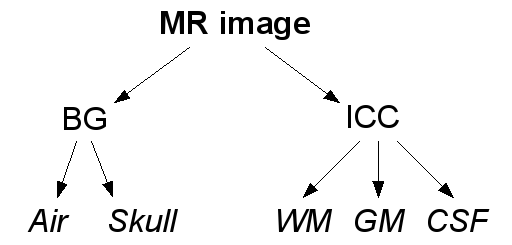
\includegraphics[width=.4\textwidth]{Images/Graphics/treeStructure.png}
  \caption{A simple tree structure of the brain}{The brain is first divided into the background (BG) and the intracranial cavity (ICC). Second the BG is dived into Air and Skull. Finally, the ICC is divided into white matter (WM), grey matter (GM) and cerebrospinal fluid (CSF)}\label{fig:treeStructure}
  \end{figure}
  
Here we continue with an intuitive description of the process. It is a brief explanation of how the image would be segmented using the hierarchical information  \ref{fig:treeStructure}. At the first iteration, the MR image will be segmented into the background (BG) and the intracranial cavity (ICC) with the EM algorithm. At the second iteration, the BG will be segmented into the air and the skull. Finally, at the last iteration, the ICC will be segmented into white matter (WM), grey matter (GM) and cerebrospinal fluid (CSF).

To formalize it, we incorporate $H$, a set of structure-specific information in Equation \ref{EMAP}. $H$ contains a lot of information like the structures of the tree which have to be segmented, an approximative size of the structure to be segmented (the Global Prior Weight) and information about which modality is the best suited to segment this structure.
\begin{equation*}
 \Phi^{(m+1)}=\operatorname*{arg\,max}_\Phi \{\sum_{k=1}^K   (p(e_{k}|Y,\Phi^{(m)},H)\operatorname*{log} p(Y,e_{k}|\Phi,H)) + \operatorname*{log} p(\Phi ,H) \} \\
\end{equation*}
%  \end{center}
 
\subsection{Summary}\label{SUMMARY}
We have shown that the EM algorithm is very flexible and can be transformed to solve a lot of segmentation problems. It is very well suited for segmentation of MR brain images and we can add a lot of informations through this algorithm to enhance the segmentation. The iterative general process is divided in two steps: the expectation (E-Step) and the maximization (the M-Step).

  \begin{itemize}
  \item \textbf{E-Step}\\  
  Estimates a soft segmentation ($p_{ik}$), given parameter $\Phi^{(m)}$. The soft segmentation creates a map of probability. Each voxel contains the probabilities that it belongs to each class. It is used for the final segmentation.
  
  \item \textbf{M-Step}\\
  Estimates $\Phi^{(m+1)}$, using the soft segmentation done in the E-Step.
  
    \begin{itemize}
    \item Estimates the intensity distribution for each tissue to be segmented.    
    \item Estimates the bias field, $\Phi^{(m+1)}$, using the soft segmentation and the intensity class distribution
    \end{itemize}
  \end{itemize}
  
The image will be segmented until the whole tree has been processed as described in section \ref{Structure}.

  \begin{figure}[ht]\centering
  \includegraphics[width=.6\textwidth]{Images/Graphics/newem.png}
  \caption{Illustration of the EM segment algorithm in Slicer}\label{fig:EMSSlicer}
  \end{figure}
  
We can also describe the segmentation process in the Figure \ref{fig:EMSSlicer}. The EM segmentation box represents the figure \ref{fig:EMAlgorithm}. To describe how it works, we use the tree structure presented in Figure \ref{fig:treeStructure}. It first segments the node $n=0$, i.e., BG and ICC. Once the EM Segmentation has converged, BG and ICC have been segmented and we move to the next node. Air and Skull will then be segmented. Following this process, all the structures of the tree will be segmented.
%
\section{Workflow in Slicer 3}
We will now present the whole segmentation workflow used in Slicer 3. It will describe all the initialisation steps done by the user, via the graphical user interface (GUI). It will also present how the whole algorithm works. We will explain why each initialisation step is important and where this information is used.
%
\subsection{User interface}\label{GUI}
It consists of a manual initialization of the parameters which are required for the segmentation on Slicer 3. The user chooses the optimal values via the GUI.

\begin{itemize}
\item \textbf{Step 1: Tree structure creation}\\
\hspace*{4 mm}We first create our problem specific tree structure for the segmentation. It will be used to define $H$ (section \ref{Structure}).
%
\item \textbf{Step 2: Atlas assignment}\\
\hspace*{4 mm}We assign to each node of the tree, i.e. each tissue to segment, the related atlas. It will be used for the spatial information (section (\ref{spatial})). It implies that an atlas for each structure to segment is needed.
%
\item \textbf{Step 3: Mutlichannel segmentation}\\
\hspace*{4 mm}We choose the images we want to use for the segmentation. As discussed in section (\ref{multichannel}), it is usefull for the multichannel segmentation since some tissues are not visible in some sequence, in some modalities.
%
\item \textbf{Step 4: Intensity normalization}\\
\hspace*{4 mm}We choose the value for the intensity normalization. We normalize the intensity of the images to be segmented, regarding the related atlas. The utility of this normalization step is presented in the next section.
%
\item \textbf{Step 5: Class definition}\\
\hspace*{4 mm}We define mean value, variance and covariance for each class and modality. It is an accurate way to initialiaze the class tissues distribution for the algorithm. It it useful because the EM algorithm only estimates the bias field but still requires information about the tissues to be segmented. Using these values, the algorithm is initialized and estimates the bias field.
%
\item \textbf{Step 6: Hierarchical parameters}\\
\hspace*{4 mm}Here we set some parameters for the hierachical segmentation. We define the utility of each target image, of the atlas for each tissue to segment and approximated the size of the tissue to be segmented. This will be stored in $H$ (section \ref{Structure}). For each tissue, $H$ knows now useful informations like which volume is the more relevant  for the class and the size that the class is supposed to be.
\par
\hspace*{4 mm}Let's take the example of the CSF. We assume a multichannel segmentation where T1 and T2 MR images are available. We give a weight of one (maximum) to the T2 target volume and zero (minimum) to the T1 target volume. It means that the only relevant information for CSF will be in the T2 volume. The algorithm will act accordingly and only use the information from T2 to perform the segmentation. It is the same for the atlas. If we set the weight of the atlas to one, the algorithm will use the spatial information. If we set it to zero, it will ignore the spatial information.
%
\item \textbf{Step 7: Registration method}\\
\hspace*{4 mm}We choose the type of registration we want. Different kind of registrations are available. The default registration method is a non-rigid registration. The rationale behind selecting a specific registration method is presented in the next section.
\end{itemize}
%
\subsection{Algorithm}
After all the initialization steps done via the GUI (section ~\ref{GUI}), we will now present the segmentation pipeline.
%
\begin{itemize}
\item \textbf{Step 1: Intensity normalization}\\
\hspace*{4 mm}The intensity of the target volumes are normalized to the value that the user chose in the GUI. The normalization works in two steps: the background is first detected in the histogram, using its low intensity and the significant number of pixels of which it is created. Then it estimates the mean values of the pixels, background excluded. Then this mean value is normalized the normalization value defined by the user via the GUI. Thus, atlas and target images have the same mean intensity (background expected). This normalization is useful if we want to use the command-line interface (i.e. if we want to run a lot of segmentations without the GUI). We just choose one atlas and all the volumes to be segmented. By normalization, the mean intensity of the target images to be segmented will be the same as in the atlas. This step is usefull because now all the target images should have the same initial parameters.
%
\item \textbf{Step 2: Image registration}\\
\hspace*{4 mm}In order for the atlas to guide the segmentation (spatial information), it has to be aligned to the target images. The transformation between the atlas and the first related target volume is evaluated during this step, using the registration method defined by the user in the GUI.
%
\item \textbf{Step 3: Spatial prior alignement}\\
\hspace*{4 mm}The transformation computed during the image registration step (step 2) is applied to all the structure-specific atlases. We finally obtain new atlases which are aligned to the images to be segmented.
%
\item \textbf{Step 4: EM Algorithm in the tree structure}\\
\hspace*{4 mm}Now, all the required initializations and preprocessing steps have been done. The whole segmentation workflow is then applied (section~\ref{SUMMARY}). A typical multichannel segmentation, using two $200x300x300$ targets volumes (T1 and T2 MR images) and segmenting five tissues, lasts around twenty minutes.
\par
The whole algorithm pipeline in summarized in Figure (\ref{algopipe}).

\begin{figure}[ht]\centering
  \includegraphics[width=0.9\textwidth]{Images/Graphics/previousalgo.png}
  \caption{Algorithm segmentation pipeline in Slicer 3}{Courtesy Pohl et al. \cite{18}. The first step of the segmentation process consists of intensity normalization. The second consists of an estimation of the transformation to apply for the registration. Third the atlases are aligned using the transformation. Finally, the EM segmentation algorithm is performed.}\label{algopipe}
  \end{figure}
  
\end{itemize}
%
\subsection{Summary}
In Slicer 3, the whole segmentation pipeline can be described as in Figure \ref{fig:Wpipeline}. There is first an initialization step, done by user via the GUI. Then, some pre-processing steps are applied in order to enhance the segmentation. Finally runs the EM pipeline to segment the MR images.

  \begin{figure}[ht]\centering
  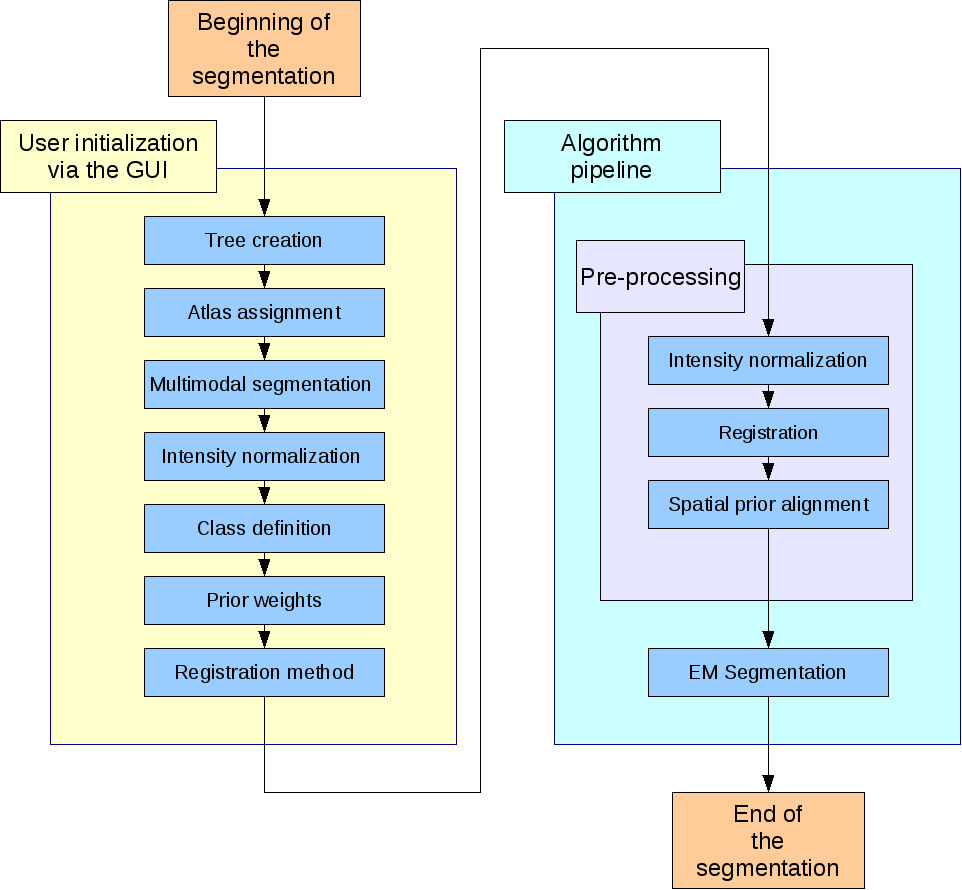
\includegraphics[width=0.8\textwidth]{Images/Graphics/wholepipeline.png}
  \caption{Flowchart of EM segmentation pipeline in Slicer 3}\label{fig:Wpipeline}
  \end{figure}

%
\section{Limitations}\label{su:limitations}
Even if the EM segmentation pipeline is robust in Slicer 3, some limitations appear.
\par
The first problem the user has to face appears during the intensity normalization step. Because of the lack of vizual feedback, it is challenging for the user to find the good normalization value. This problem will be discussed in section \ref{intensitynormalizationddd}.
\par
The second problem is directly linked to the EM algorithm. As the maximization method is a local one, the class distribution, which are used for the initialization of the algorithm has to be well defined. So far, we have no possibilities to know how accurate our definition of the class is. This problem will be discussed in details in section \ref{sec:tables}.
\par
Another problem appears at the same steps. The actual method for defining means and variances for each class appears not as efficient as we want it to be. This problem will be discussed in details in section \ref{sec:CDS}.
\par
Moreover, if the user is not familiar with the EM segment algorithm, defining good hierarchical parameters can be challenging. In section \ref{GPSPDGSPGS} we will provide a tool to help the user.
\par 
The last problem we encounter appears after the initialization, during the preprocessing. Only one preprocessing  step (intensity normalization) is done on the target images before the atlases are registered to it. Since the EM algorithm is targeted to work on MR images, bias field is a recurrent problem. Performing the registration without bias correction might affect the results of the registration. This problem will be discussed in details in section \ref{biasfieldcorrectionregistration}.

%
\par
In this chapter, we have described the EM segmnetation algorithm and its implementation in Slicer 3. We have concluded this the limitations of the current implementation. In the next chapter we will propose some solutions and describe them in details.